\documentclass[a4paper,man,natbib]{apa6}

\usepackage[english]{babel}
\usepackage[utf8x]{inputenc}
\usepackage{amsthm}
\usepackage{amsmath}
\usepackage{amssymb}
\usepackage{mathtools}
\usepackage{graphicx}
\usepackage[colorinlistoftodos]{todonotes}
\usepackage{url}

\newcommand{\C}{\mathbb{C}}  % Complex
\newcommand{\R}{\mathbb{R}}  % Real
\newcommand{\Z}{\mathbb{Z}}  % Integers

\title{$ \C $omplex Geometry \& $ \C $onformal Maping}
\shorttitle{geometry \& mapping}
\author{ $\C $ason Konzer}
\date{April 2021}
\affiliation{University of Michigan}

\abstract{In this paper we will explore aspects of complex geometry and mapping fundamentals. 
The beginning of this paper will give background on the funadmental geometric structure of complex numbers. 
Following we will dive into rectangular and polar coordinates, mappings from domain to co-domain, and the way regions are defined.
A breif look at curve parameterization will be used as it will be imporntant with respect to conformal maps. 
With geometric fundamentals set, we will define holomorphic/analytic functions, then explore transformations within the complex plane.
Focusing on locally invertable functions, we will prove such invertability in a few cases. 
At this point the context is set and the discussion with shift towards conformal mapping. 
We will conclude this paper by extending conformal mapping into real world applications.}

\begin{document}
\maketitle

\section{Introduction \& Background}
\label{sec: Before we Start}

Complex functions are mappings from one complex valued variable to another. In general the domain and co-domain are $ \C $.
Throughout this paper we will reference $ z,w \in \C $ such that $ z $ is some input from our domain, and $ w $ is the respective output in the co-domain. 
It is often the case that we consider complex valued functions in which the domain and co-domain do not span the whole complex plane. 
To fomalize this concept we will consider two regions $ Z $ and $ W $ such that $ z \in Z $ and $ w \in W $, where $ Z,W \subseteq \C $. 
Here, $ Z $ is the domain, $ W $ the co-domain, $ z $ the input, and $ w $ the output, or image. Following symbolically \dots

\begin{center}

      $ f: Z \to W $ ; $ z \mapsto w $ ; $ f(z) = w $ 

\end{center}



A complex valued variable is formed from 2 real valued numbers, with one representing a real and the other an imaginary part.
Following this representation, $ \C $ is very similar to $ \R \times \R $, or $ \R^2 $.  
To see this similarity it is helpful to view the rectangular form of the Complex number. Here, $z = x + iy$ where $x,y \in \R$. 
In this context, and continuing throught this paper, $ i $ denotes the imaginary number, where $ i = \sqrt{-1} $ and $ i^2 = -1 $.
We can now see that $ f $ is a sum of two functions. For this paper we will consider functions $u$ and $v$ \dots

\begin{center}

      $ u,v: (\R \times \R) \to \R $ ; $ f(x+iy) = u(x,y) + iv(x,y) $ 

\end{center}

It is common to dissolve complex numbers into these real and imaginary parts. Here $ x \coloneqq Re(z) $ and $ y \coloneqq Im(z) $, where $ Re $ denotes the real part and $ Im $ the imaginary.
Similarlly, $ \mu \coloneqq Re(f(z)) = Re(w) $ and $ \nu \coloneqq Im(f(z)) = Im(w) $, coming full circle \dots

\begin{center}

      $ f : x,y \mapsto \mu,\nu $ ; $ f(z) = f(x+iy) = u(x,y) + iv(x,y) = \mu + i\nu = w $ \\
     *Figure 1 is provided to illustate this concept with a simple translation function.

\end{center}

At this point it is worth noting a few other aspects of the complex numbers, although they will not all be necessecary for the following discussion. 

\begin{itemize}

\item The complex conjugate, $ \bar{z} $, is defined as $ \bar{z} \coloneqq x - iy $ where $ z = x +iy $, 
This operation switches the sign of $ Im(z) $ and has a unique geometric property of changing the direction of an angle $ \vartheta $ 
between the vector pointing from the origin in the complex plane, 0, to $z$ and the positive real axis.

\item The magnitude, or norm, of $ z $, given by $ |z| $, is defined as $ |z| \coloneqq \sqrt{x^2 + y^2} $.
As consequence, we can notice $ x \coloneqq  |z|\cos(\vartheta) $, $ y \coloneqq  |z|\sin(\vartheta) $, and $ \vartheta \coloneqq  \tan^{-1}(\frac{y}{x}) $

\item Additionally, $ z\bar{z} = (x + iy)(x - iy) = x^2 +ixy - ixy - i^2y^2 = x^2 + y^2$  We can now see a new definition for the norm arise, as well as a relation to the conjugate.
$ |z| = \sqrt{z\bar{z}} = |\bar{z}| $. Figure 2 summarizes these first points.

\item Lastly, we can define the polar representation of $ z $ in terms of its norm, and $\vartheta$, refered to as its argument,  $ z \coloneqq  |z|e^{i\vartheta} $. This is derived from the trigonometric definitions for $ x $ and $ y $.  

\end{itemize}

It is often common to consider the regions $ Z $ and $ W $ in terms of curves $ \gamma $ and $ \Gamma $.
There are a few options for where the elements $ z $ and $ w $ are allowed to be. If elements in the given region are allowed to lie on the respective curve, it is consider closed.
Conversly the region is considered open given the elements are not allowed on the curve. 
In specific, $ Z $ is considered open given each element $ z \in Z $ can be surrounded by an open disc of radius $ r \gneq  0 $.
Elements of $ Z $ and $ W $ can then lie inside/outside the curve, or possibly inbetween some 2 curves  $ \gamma_{1},\gamma_{2} $ or $ \Gamma_{1},\Gamma_{2} $
We can then paramaterize these curves in terms of $ t $ where $ \gamma(t), \Gamma(t) $ trace out the respective curves given $ t_{i} \leq t \leq t_{f} $
In the case of a loop, $ t_{f} = t_{i} + 2\pi $ as the curve will end where it started, making one full revolution around a central point. 
In other circumstances $ t_{f} = t_{i} + 2k\pi $ where $ k \in \Z $. A positive $ k $ represents an anti-clockwise loop while a negaitve $ k $ represents a clockwise loop. 
$ k $ is refered to as the winding number. There is no limit to the number of curves that define a region, or that lie in a region. 
Figures 3 and 4 take a moment to show this visually. 
\\
We will take a breif detour to now define a few imporntant terms. 
A function $ f $ is \textit{differentiable} provided that the limit below exits, given $ \zeta $ lives in the domain $ Z $.

\begin{center}

      $ f'(\zeta) \coloneqq \lim_{z \to \zeta} \frac{f(z) - f(\zeta)}{z - \zeta} $ 

\end{center}

We will then define the image of $ \zeta $ to be $ \omega $, where the co-domain is $ W' $

\begin{center}

      $ f': Z \to W' $ ; $ \zeta \mapsto \omega $ ; $ f'(\zeta) = \omega $ ; $ \zeta \in Z $ ; $ \omega \in W' $

\end{center}

Following nicely, $ f $ is considered \textit{holomorphic} given $ \forall \zeta \in Z $, $ \exists \omega \in W' $, 
such that no $ \zeta $ falls on a parametric curve $ \gamma(t) $ used to define $ Z $, hense $ Z $ must be an open region.
Keep in mind that this image $ \omega $ is not the same as the image $ w $, in fact because $ \omega $ is the image of the derivative, it is best thought of a tanget vector. 
In complex analysis, the term \textit{holomorphic} is often used interchangeable with the term \textit{analytic}.
Although, in general, \textit{analytic} is the stronger of the two. 
The difference is that \textit{analytic} implies that $ f $ has a power series representation.
We will not dive deeply into the reasoning, but because the nature of complex variables, 
all \textit{analytic} functions are \textit{holomorphic}, and all \textit{holomorphic} functions are \textit{analytic}.
Recalling from before, we know $ f $ is equivalent to $ u +iv $, where each function $ f,u,v $ is input the same complex number, $ z $, of two real variables, $ x $ and $ y $. 
To test whether a function is \textit{analytic}, we use a system of equations coined the Cauchy-Reimann $ (C.R.) $ equations, to honor two of the mathematicians, 
Cauchy and Reimann, who have done some of the most piviotal work with developing and elaborating upon them. They are as follows \dots

\begin{center}

      $ f(u,v) = u(x,y) +iv(x,y) $ ; $ f'(u(x,y),v(x,y)) = $$ \frac{\delta f}{\delta u} \frac{\delta u}{\delta x} + \frac{\delta f}{\delta v} \frac{\delta v}{\delta x} + 
      \frac{\delta f}{\delta u} \frac{\delta u}{\delta y} + \frac{\delta f}{\delta v} \frac{\delta v}{\delta y} $ 
      \\
      $ (C.R.) $ $ u_{x} = v_{y} $ ; $ v_{x} = -u_{y} $ 
      \\
      $ f'(u,v) = u_{x} + v_{x} + u_{y} + v_{y} = u_{x} + v_{x} = v_{y} - u_{y} $
      \\
      It is not uncommon to see $ f' = f_{x} $ as $ f_{x} = u_{x} + v_{x} $

\end{center}

Following the $ (C.R) $ equations, we can examine the examine the derivative of the function $ f $, and notice that there are two interpretations of the solutions.
In the first listed, we can see that the the derivative is interpreted as the sum of the real contribution from the input, $ Re(z) = x $, seen in the outputs, $ w = \mu + i\nu $.   
Adversly, in the equivalent definition, we see that the derivative is defined as the diffrence of the imaginary contribution, $ Im(z) = y $, of $ \nu $ and $ \mu $.
For the $ (C.R) $ equations to hold, we must verify both that $ u_{x} = v_{y} $, and $ v_{x} = -u_{y} $, in whice case $ f $ is indeed \textit{analytic}. \\
* Figure 5 offers a geometric proof of the $ (C.R) $ equations. 
What is particularlly intresting here is that we can see a prevelant scalling from $ |\vartriangle x| $ to $ |\vartriangle f_{1}| $ and from $ |\vartriangle y| $ to $ |\vartriangle f_{2}| $,
of equal factor; And both $ \vartriangle x $ and $ \vartriangle y $ experience a rotation of $ \vartheta $ to $ \vartriangle f_{1} $ and $ \vartriangle f_{2} $ respectively. 

\section{Geometric Mapping}
\label{sec: Mapping}

\subsection{$ M\ddot{o}bius $ $ Transformations $ $ \& $ $ Inversion $}

A $ m\ddot{o}bius $ transformion is uniquely defined by a culmination of 4 other transformations. One can consist of a part translation, magnification, rotation, and inversion.
\\
A translation a vector shift. Because we are working in the complex plane, this is best thought of as a function, call it $ T $, that 
moves a complex variable $ z $ some distance $ \beta $ where $ z = x + iy $ and $ \beta = a + ib $ Functionally \dots

\begin{center}

      $ T(z) = T(x + iy) = (x + a) + i(y +b) = w $ 

\end{center}

Magnification and rotation are combined into a transformation called a dialation due to the nature of complex numbers. 
It is useful to use the polar representation when thinking about this kind of manipulation. 
At this point it is relevant to note that when multiplying two complex numbers, the mechanics are such that the norms are mulitplied but the arguments are added. 
Considering the vector pointing to $ z $, and multiplying $ z $ by some complex number $ \alpha $, $ z $ will be scaled by $ Norm(\alpha) $, and rotated by $ Arg(\alpha) $.
Letting $ \alpha = |\alpha |e^{i\varphi} $, and remembering the polar representation of $ z $ as $ z = |z|e^{i\vartheta} $, we can define a function D \dots

\begin{center}

      $ D(z) = \alpha z $ ; $ D(|z|e^{i\vartheta}) = |\alpha ||z|e^{i(\vartheta + \varphi)} = w $ 

\end{center}

As a side note, a magnification is seen when we set $ Arg(\alpha) $, or $ \varphi $ equal to 0, as $ \vartheta + 0 = \vartheta $ and no rotation will occur.
Similarly, a rotation will occur given $ Norm(\alpha) $, or $ |\alpha| $ equal to 1, as $ 1|z| = |z| $ and no magnification will occur.
Of course, in order for either scenario to create a transformation, we must have $ |\alpha| \neq 1 $ or $ \varphi \neq 2k\pi $, with $ k \in \Z $, else $ z $ will remain in its origional positon.
\\
Lastly, an inversion will scale and rotate a complex variable, without any other factors than $ z $ itself.
Letting $ I $ be an inversion, $ I(z) \coloneqq \frac{1}{z} = z^{-1}$. In polar form, 

\begin{center}

      $ I(|z|e^{i\vartheta}) = \frac{1}{|z|e^{i\vartheta}} = \frac{e^{-i\vartheta}}{|z|} = w $ 

\end{center}

At this point it should be clear that each one of these transformations are locally invertible. 
The image of a translation can be brought by by switching the signs for both $ a $ and $ b $, 
a dialation by multiplying $ w $ by a variable $ \frac{e^{-i\varphi}}{|\alpha|} $, and an inversion is inverted by reapplying the inversion function itself.
We know that $ f : z \mapsto w $ and for the inverse, $  f^{-1}: w \mapsto z $. Formally we write ... 

\begin{itemize}

      \item For Translation: $ T(z) = z + \beta = w $ ; $ T^{-1}(w) = w - \beta = z $ ; $ (T^{-1} \circ  T)(z) = (z + \beta) - \beta = z  $
      
      \item For Dialation: $ D(z) = \alpha z = w $ ; $ D^{-1}(w) = \frac{w}{\alpha} = z $ ; $ (D^{-1} \circ  D)(z) = \frac{(\alpha z)}{\alpha} = z $
      
      \item For Inversion: $ I(z) = \frac{1}{z} = w $ ; $ I^{-1}(w) = \frac{1}{w} = z $ ; $ (I^{-1} \circ  I)(z) = \frac{1}{(\frac{1}{z})} = z $
      
\end{itemize}

We can now think of a $ m\ddot{o}bius $ transformation as the composition of various magnifications, dialations and inversions. 
As each of these transformations are themselves invertible the $ m\ddot{o}bius $ transformation is inveritable as well. For clarity, assume a function, $ M $,
is a $ m\ddot{o}bius $ transformation that first inverts $ z $, and thereafter applies a translation before a final dialation. Thus,

\begin{center}

      $ M(z) = (D \circ (T \circ I))(z) $ ; $ M^{-1} = (I^{-1} \circ (T^{-1} \circ D^{-1}))(z) $ ; \\
      $ (M^{-1} \circ M)(z) = (I^{1} \circ ((T^{-1} \circ D^{-1})) \circ (D \circ (T \circ I)))(z) $ \\ 
      $ = (I^{-1} \circ (T^{-1}) \circ (T \circ I))(z) = ((I^{-1}) \circ (I))(z) = z $ \\
      *Figure 6 is provided to illustate this example by applying transforms on a point $ z $.

\end{center}

At this point it is appropriate to introduce the explict formula for a $ m\ddot{o}bius $ transformation.

\begin{center}

      $ M(z) = \frac{az + b}{cz + d} $ ; given $ a,b,c,d \in \C $ and $ ad - bc \neq 0 $

\end{center}

By the method of substitution, $ M(z) = w $, we can additionally solve for an explicit inverse function, $ M^{-1}(w) = z $

\begin{center}

      $ M(z) = \frac{az + b}{cz + d} = w $ $ \Rightarrow $ $ wcz + wd = az + b $ $ \Rightarrow $ $ z(wc - a) = b - wd $ $ \Rightarrow $ $ z = \frac{b - wd}{wc - a} $
      $ M^{-1}(w) = z = \frac{b - wd}{wc - a} $ ; $ (M^{-1} \circ M)(z) = \frac{b - \frac{az + b}{cz + d}d}{\frac{az + b}{cz + d}c - a} 
      = \frac{\frac{b(cz + d) - d(az + b)}{cz + d}}{\frac{c(az + b) - a(cz + d)}{cz + d}} = \frac{\frac{bcz + bd - adz - bd}{cz + d}}{\frac{acz + bc - acz - ad}{cz + d}} 
      = \frac{(bcz - adz)(cz +d)}{(bc - ad)(cz + d)} = \frac{z(bc - ad)}{(bc - ad)} = z $ 

\end{center}

One technical term used to describe a $ m\ddot{o}bius $ transformation is linear fractional transformation. 
This verbage stems from the fact that the numerator, $ az + b $, and the denomenator, $ cz + d $, are both of linear form.
Parsing $ M(z) $ with a close eye, we can see that there is one zero, where $ z = \frac{-b}{a} $ and one pole, where $ z = \frac{-d}{c} $.
From here we digress to Figure 7, characterizing the $ m\ddot{o}bius $ transformation as a map from a point $ z $ on a Reimann sphere to a point $ w $.
Because the domain and co-domain are both the sphere, this can be thought of as a self map. It is from this interpretation that stereographic projection was set. 

\subsection{$ Conformal Maps $}

With invertible functions under our belt, there are two major realizations to come to.
First, an \textit{analytic} function must be injective, one-to-one, in order hold uniqueness. 
If this were not the case we could not know what input produced an image when trying to pull it back to the domain.
Second, we will assume that the inverse function from real numbers, and the corresponding derivative of the inverse function translates to complex numbers.
Letting $ f^{-1}(z) = \xi $, We can see there is a well defined inverse function as $ f(z) = w $ ; $ z = \xi(w) $, $ \dots $ 

\begin{center}

      $ f(\xi(z)) = z $ ; $ f'(\xi(z))\xi'(z) = 1 $ ; $ \xi'(z) = \frac{d}{dz}f^{-1}(z) = \frac{1}{f'(\xi(z))} $

\end{center}

This equation thus implies that $ f' \neq 0 $ as $ \xi = f^{-1}(z) $ is to be differentiable. We now have the full critera for conformal maps. 
A conformal map is a complex valued function such that it is \textit{analytic} and locally invertible. 
This requires that the function both satisfies the $ (C.R) $ equations, and it's derivative is non-zero, within the region of concern. 
Angle preservation was hitied at earlier when exploring the $ (C.R) $ equations, and in fact, all functions that satisfy such equations, including conformal maps of course, are angle preservating.
But what exactly does it mean it be angle preserving? Figure 8 is included to illustrate this.
Consider two paths within the region $ Z $, where $ f $ is a conformal map. Because of the path parameterization, they are directional and to be traversed only one way. 
It then follows that images two paths within $ W $ will also be directional, and as $ f $ is a conformal map, 
they will have the same angle between them at crossings points $ w $ in $ W $, when compared with crossing points $ z $ in $ Z $.
Here, we let our friendly function $ f $ map $ \gamma $ to $ \Gamma $. Symbolically \dots

\begin{center}

      $ f : Z \to W $ ; $ z \mapsto w $ : $ \gamma \mapsto \Gamma $ ; $ f(\gamma(t)) = \Gamma(t) $ | $ t_{i} \leq t \leq t_{f} $

\end{center}

The fact that makes these mappings work, is that the same function $ f $ will also map the tangent vectors on the curve for any given t within its scope.
To find these tangent lines in the region $ W $, we will need to consider $ \frac{\delta}{\delta t}f(\gamma(t)) $, or $ \Gamma'(t) $.
But first let us consider the angle $ \theta $ that occurs between $ \gamma_1 $ and $ \gamma_2 $. 
Because it is the derivative at some point $ z $, at the intersection of $ \gamma_1 $ and $ \gamma_2 $, that 
defines the tangent vectors, we will need to consider $ \gamma'_1(t) $ and $ \gamma'_2(t) $. These two derivatives will 
point in the directon the paths are moving when they cross $ z $. 
An imporntant formula used to determine similarity of vectors will be used to solve for $ \theta $.
Considering two vectors $ \jmath $ and $ \ell $, we have \dots

\begin{center}

      $ \theta = cos^{-1}(\frac{\jmath  \cdot \ell }{\left\lVert \jmath \right\rVert \left\lVert \ell  \right\rVert })$

\end{center}

Now we can sub in the two vectors we obtained from our $ \gamma $ function. (For simplification, time derivative will be represented with dot notation). \dots

\begin{center}

      $ \theta = cos^{-1}(\frac{\dot{\gamma}_1  \cdot \dot{\gamma}_2 }{\left\lVert \dot{\gamma}_1 \right\rVert \left\lVert \dot{\gamma}_2  \right\rVert })$

\end{center}

Before trying to simplify any further, it becomes useful to consided the images of these curves, and to introduce the Jacobian matrix, $ \mathcal{J} $, as $ \dot{\Gamma} $ = $ \mathcal{J}_f\dot{\gamma}$, where \dots

\begin{center}

      $ \mathcal{J}_f = \begin{bmatrix}
        f_{xx} & f_{xy}\\
        f_{yx} & f_{yy}
        \end{bmatrix} $ ; 
      $ \dot{\gamma} = \begin{bmatrix}
        \dot{\gamma}_x\\
        \dot{\gamma}_y
        \end{bmatrix} $ ;   
      $ \dot{\Gamma} = \begin{bmatrix}
        f_{xx} & f_{xy}\\
        f_{yx} & f_{yy}
        \end{bmatrix}
        \begin{bmatrix}
        \dot{\gamma}_x\\
        \dot{\gamma}_y
        \end{bmatrix} 
        = \mathcal{J}_f\dot{\gamma}$
      
\end{center}

We now have an explicit solution to solve $ \dot{\Gamma} $ for it's relative tangent vector on the path $ \Gamma(t) $, in $ W $.
In order to check for angle preservation, we will need to look at both $ \dot{\Gamma}_1 $ and $ \dot{\Gamma}_2 $.
We will use the same function as before for the angle between two vectors, but consider this angle as $ \Theta $ \dots

\begin{center}

      $ \Theta = cos^{-1}(\frac{\mathcal{J}_f\dot{\gamma}_1 \cdot \mathcal{J}_f\dot{\gamma}_2}{{\left\lVert \mathcal{J}_f\dot{\gamma}_1 \right\rVert \left\lVert \mathcal{J}_f\dot{\gamma}_2  \right\rVert }}) $
      $ = cos^{-1}(\frac{(\mathcal{J}_f\dot{\gamma}_1)^T(\mathcal{J}_f\dot{\gamma}_2)}{\sqrt{{(\mathcal{J}_f\dot{\gamma}_1)^T(\mathcal{J}_f\dot{\gamma}_1)(\mathcal{J}_f\dot{\gamma}_2)^T(\mathcal{J}_f\dot{\gamma}_2)}}})$
      $ = cos^{-1}(\frac{\dot{\gamma}_1^T(\mathcal{J}_f^T\mathcal{J}_f)\dot{\gamma}_2}{\sqrt{\dot{\gamma}_1^T(\mathcal{J}_f^T\mathcal{J}_f)\dot{\gamma}_1\dot{\gamma}_2^T(\mathcal{J}_f^T\mathcal{J}_f)\dot{\gamma}_2}})$
      $ = cos^{-1}(\frac{\dot{\gamma}_1^T\dot{\gamma}_2}{\sqrt{\dot{\gamma}_1^T\dot{\gamma}_1\dot{\gamma}_2^T\dot{\gamma}_2}})$
      $ = cos^{-1}(\frac{\dot{\gamma}_1^T\dot{\gamma}_2}{\left\lVert \dot{\gamma}_1 \right\rVert \left\lVert \dot{\gamma}_2  \right\rVert })$ \\
      Now what a suprise it it, \\
      $ \Theta = cos^{-1}(\frac{\dot{\gamma}_1  \cdot \dot{\gamma}_2 }{\left\lVert \dot{\gamma}_1 \right\rVert \left\lVert \dot{\gamma}_2  \right\rVert }) = \theta $
      
\end{center}

It has come to our attention that angles are preserved as we arrive at $ \theta = \Theta $.
Although in this walk though we make the assumption that $ \mathcal{J}_f^T\mathcal{J}_f = 1 $. 
This does indeed happen in a few situtaions. $ \mathcal{J}_f $ could be the identity matrix, or some scalar multiple of it, as well as a rotational matrix. \dots

\begin{center}

$ \mathcal{J}_f = \begin{bmatrix}
        1 & 0\\
        0 & 1
\end{bmatrix} $ ;
$ \mathcal{J}_f = \begin{bmatrix}
      \sigma  & 0\\
      0 & \sigma 
\end{bmatrix} $ ;
$ \mathcal{J}_f = \begin{bmatrix}
      cos(\phi) & sin(\phi)\\
      -sin(\phi) & cos(\phi)
\end{bmatrix} $

\end{center}

There are indeed many applications that come from the logic behind confromal mapping. 
Some of these consider boundary conditions, such as the Dirchlet and Neumann boundary conditions that follow conformal maps. 
Other applications include cartography, traditional map making, such as creating the best flat map of the globe. 
In computer science conformal geometry is quite crucial for image manipulation and distortion, while perserving angles. 
In physics, conformal maps and complex alaysis provides an "elevated" perspective on many problem and is highly related to the Laplacian. 
And of course there is the applications in pure mathematics and joy; hence, for the last Figure, I will leave an artpice by M.C. Escher which utilizes a conformal map. 

\newpage
\subsection{References}

      Crane, K. (2017). Conformal Geometry Processing [Recorded Lecture]. Retrieved From
\url{https://www.youtube.com/watch?v=g0nY5VM1PSU}
\\
      Faculty of Khan. (2020). Conformal Mapping in Complex Variables [Recorded Lecture]. Retrieved From
\url{https://www.youtube.com/watch?v=g6gFdyqlwWE}
\\
      Gross, H. (1972). Part I: Complex Variables, Lec 3: Conformal Mappings [Recorded Lecture]. Retrieved From
\url{https://www.youtube.com/watch?v=s1DFa1dCss0&t=24s}
\\
      Hammack, R. (2007). A Geometric View of Complex Trigonometric Functions. \textit{The College Mathematics Journal, 38}(3).
\\
      Olver P. (2020). Complex Analysis and Conformal Mapping [PDF Lecture Notes]. Retrieved From
\url{http://www-users.math.umn.edu/~olver/ln_/cml.pdf}
\\
      Paul, A. (2017). Cauchy Riemann Equations [Recorded Lecture]. Retrieved From
\url{https://www.youtube.com/watch?v=PWG78CD7xMk}
\\
      Robinson, M. (2020). Moebius transformations [Recorded Lecture]. Retrieved From
\url{https://www.youtube.com/watch?v=wTOHJprHXzs}
\\
      Robinson, M. (2020). Conformal mappings [Recorded Lecture]. Retrieved From
\url{https://www.youtube.com/watch?v=xbDKCNvMB78&list=PLSekr_gm4hWIQXnDGEsSubbmA0JPueTOx&index=28}
\\
      Robinson, M. (2020). Conformal mappings of boundary conditions [Recorded Lecture]. Retrieved From
\url{https://www.youtube.com/watch?v=SsWfG92ER40&list=PLSekr_gm4hWIQXnDGEsSubbmA0JPueTOx&index=24}
\\
      Romik, D. (2020). Complex Analysis Lecture Notes [PDF Lecture Notes]. Retrieved From
\url{https://www.math.ucdavis.edu/~romik/data/uploads/notes/complex-analysis.pdf}
\\
      Rosales R., Andre Nachbin, Jeremy Orloff, and Jorn Dunkel. (2020). 18.04 Complex analysis with applications [PDF Lecture Notes]. Retrieved From
\url{https://math.mit.edu/classes/18.04/Notes/1804_Complex_Analysis_with_Applications20200203.pdf}
\\
      Smit B. and Lenstra H. (2003). The Mathematical Structure of Escher’s Print Gallery. \textit{Notices of The AMS, 50}(4).
\\
      The Math Coach. (2019). Conformal Mapping | Mobius Transformation | Complex Analysis 22 [Recorded Lecture]. Retrieved From
\url{https://www.youtube.com/watch?v=48aerHs9wL0}

% Commands to include a figure:

\begin{figure}

      \centering
      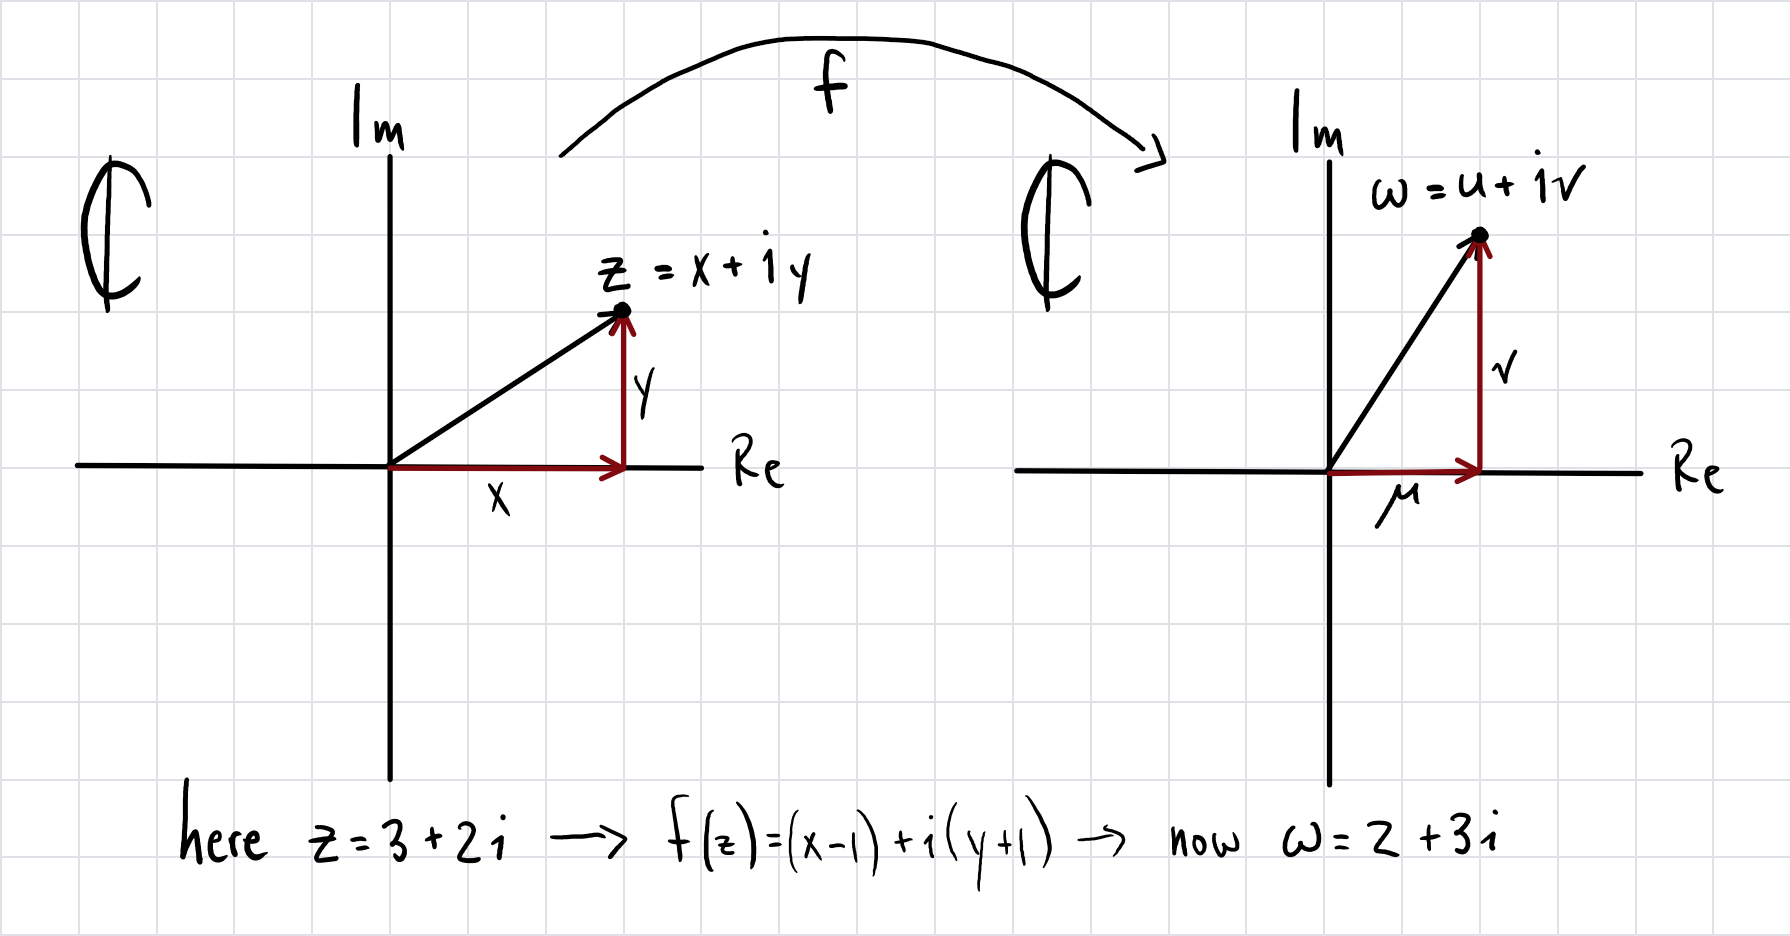
\includegraphics[width=1\textwidth]{C:/Users/cason/OneDrive - Umich/Math/CV/Project (Geometry & Mapping w C)/Rectangular Map.png}
      \caption{\label{C:/Users/cason/OneDrive - Umich/Math/CV/Project (Geometry & Mapping w C)/Rectangular Map.png}
      Illustrated here is a function $ f $, mapping a point $ z \in \C $ to $ w \in \C $ where $ f(z) = z -1 +i $.}

\end{figure}

\begin{figure}


      \centering
      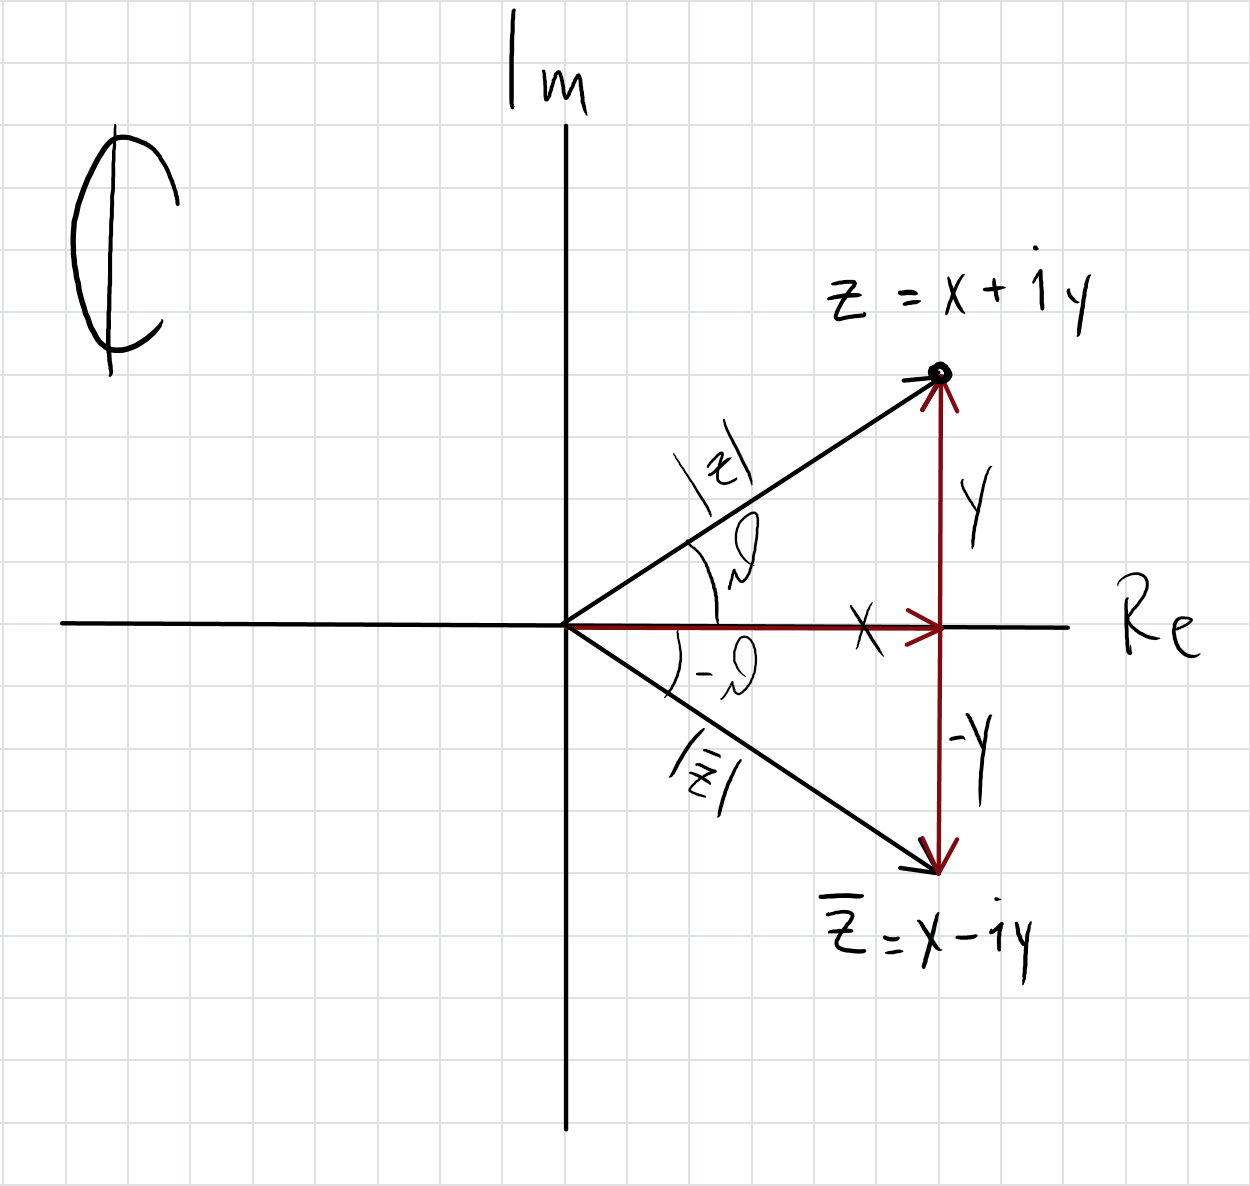
\includegraphics[width=1\textwidth]{C:/Users/cason/OneDrive - Umich/Math/CV/Project (Geometry & Mapping w C)/Polar Coordinates.png}
      \caption{\label{C:/Users/cason/OneDrive - Umich/Math/CV/Project (Geometry & Mapping w C)/Polar Coordinates.png}
      Illustrated here are points $ z, \bar{z} \in \C $, with $ \vartheta $, $ -\vartheta $  representing the argument, and $ |z| $, $ |\bar{z}| $ representing the norm of $ z, \bar{z} $ respectively.}

\end{figure}

\begin{figure}

      \centering
      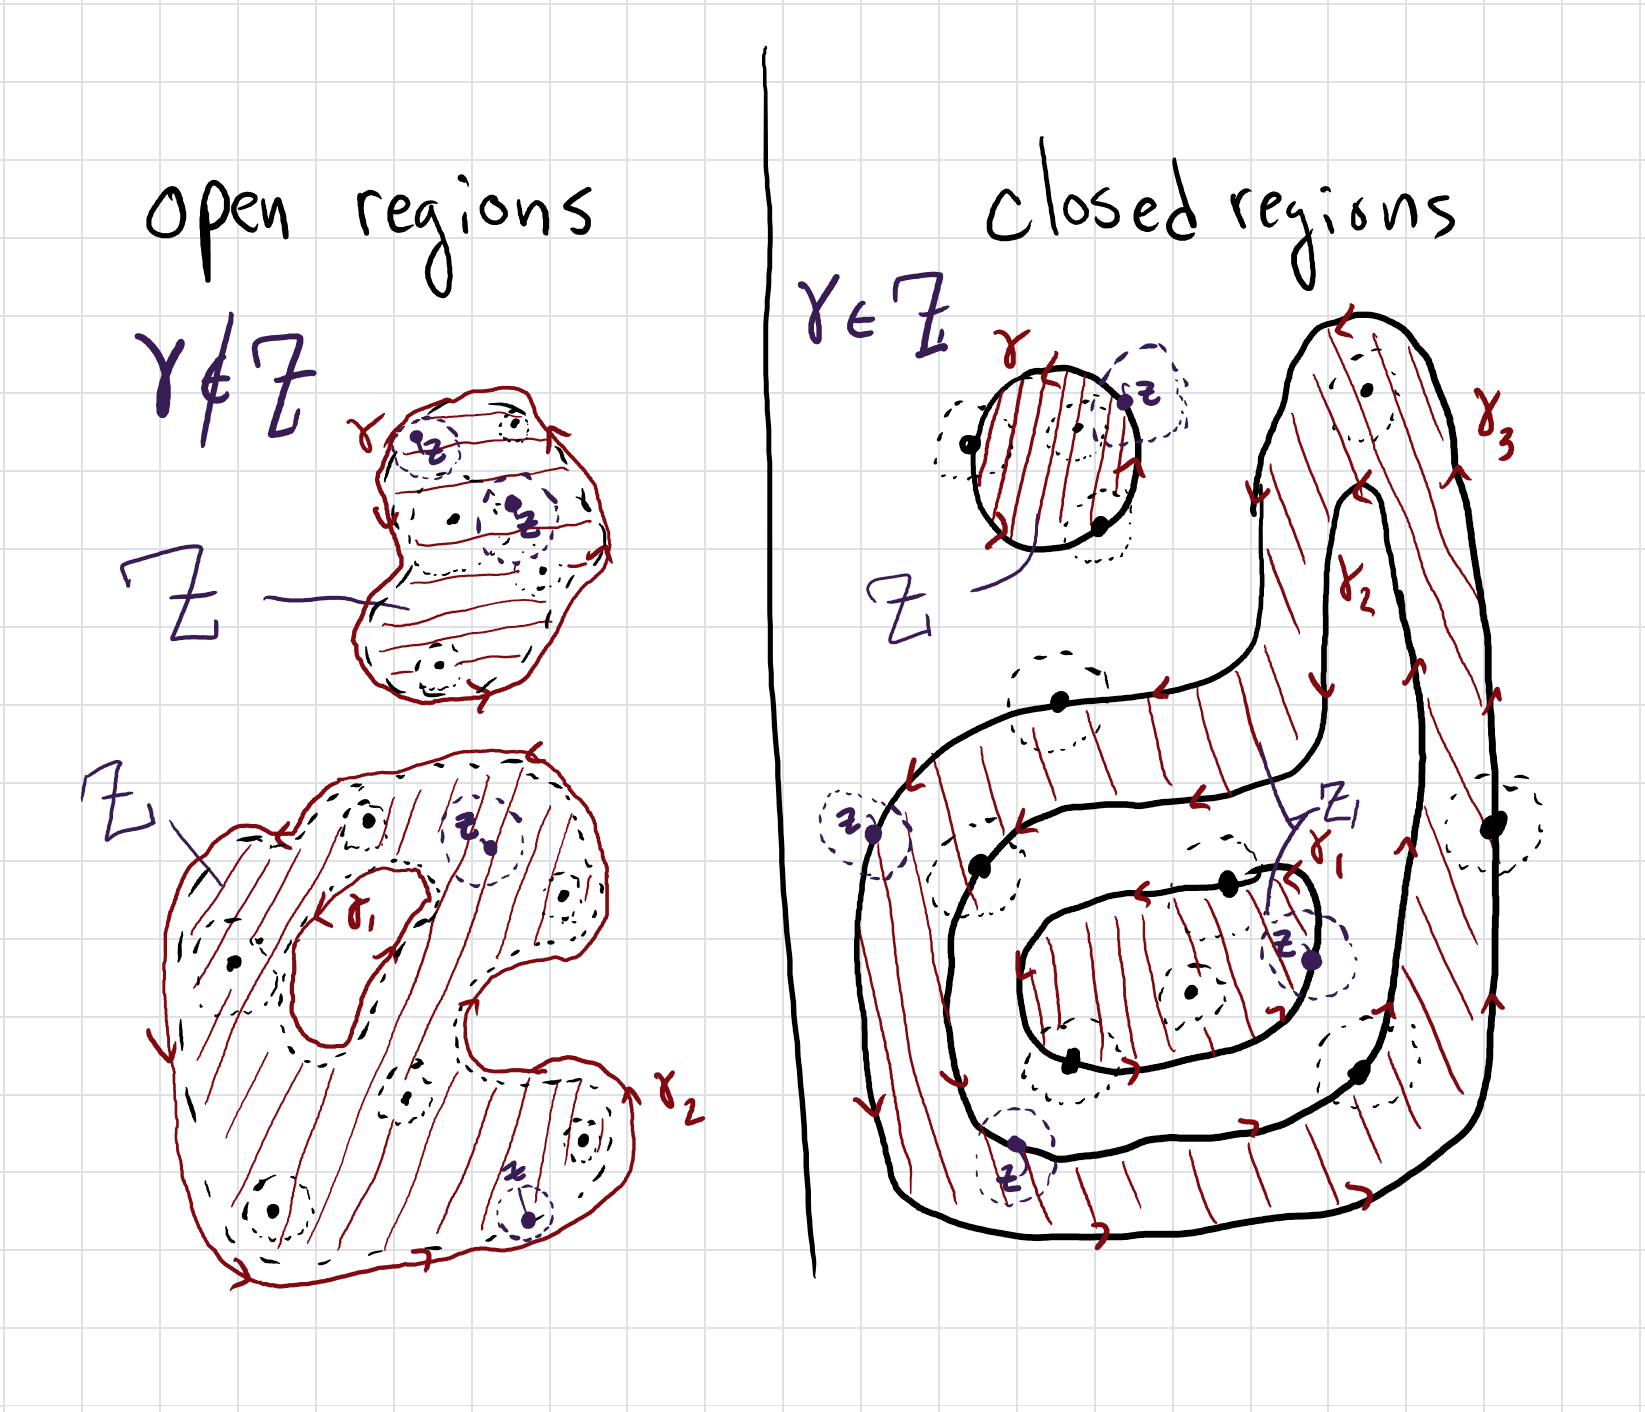
\includegraphics[width=1\textwidth]{C:/Users/cason/OneDrive - Umich/Math/CV/Project (Geometry & Mapping w C)/Regions.png}
      \caption{\label{C:/Users/cason/OneDrive - Umich/Math/CV/Project (Geometry & Mapping w C)/Regions.png}
      Illustrated here are closed regions where a point $ z $ may lie on the parametric curve $ \gamma $, 
      and open regions where $ z $ can always be surronded by an open disc, as it cannot lie on $ \gamma $.}

\end{figure}

\begin{figure}

      \centering
      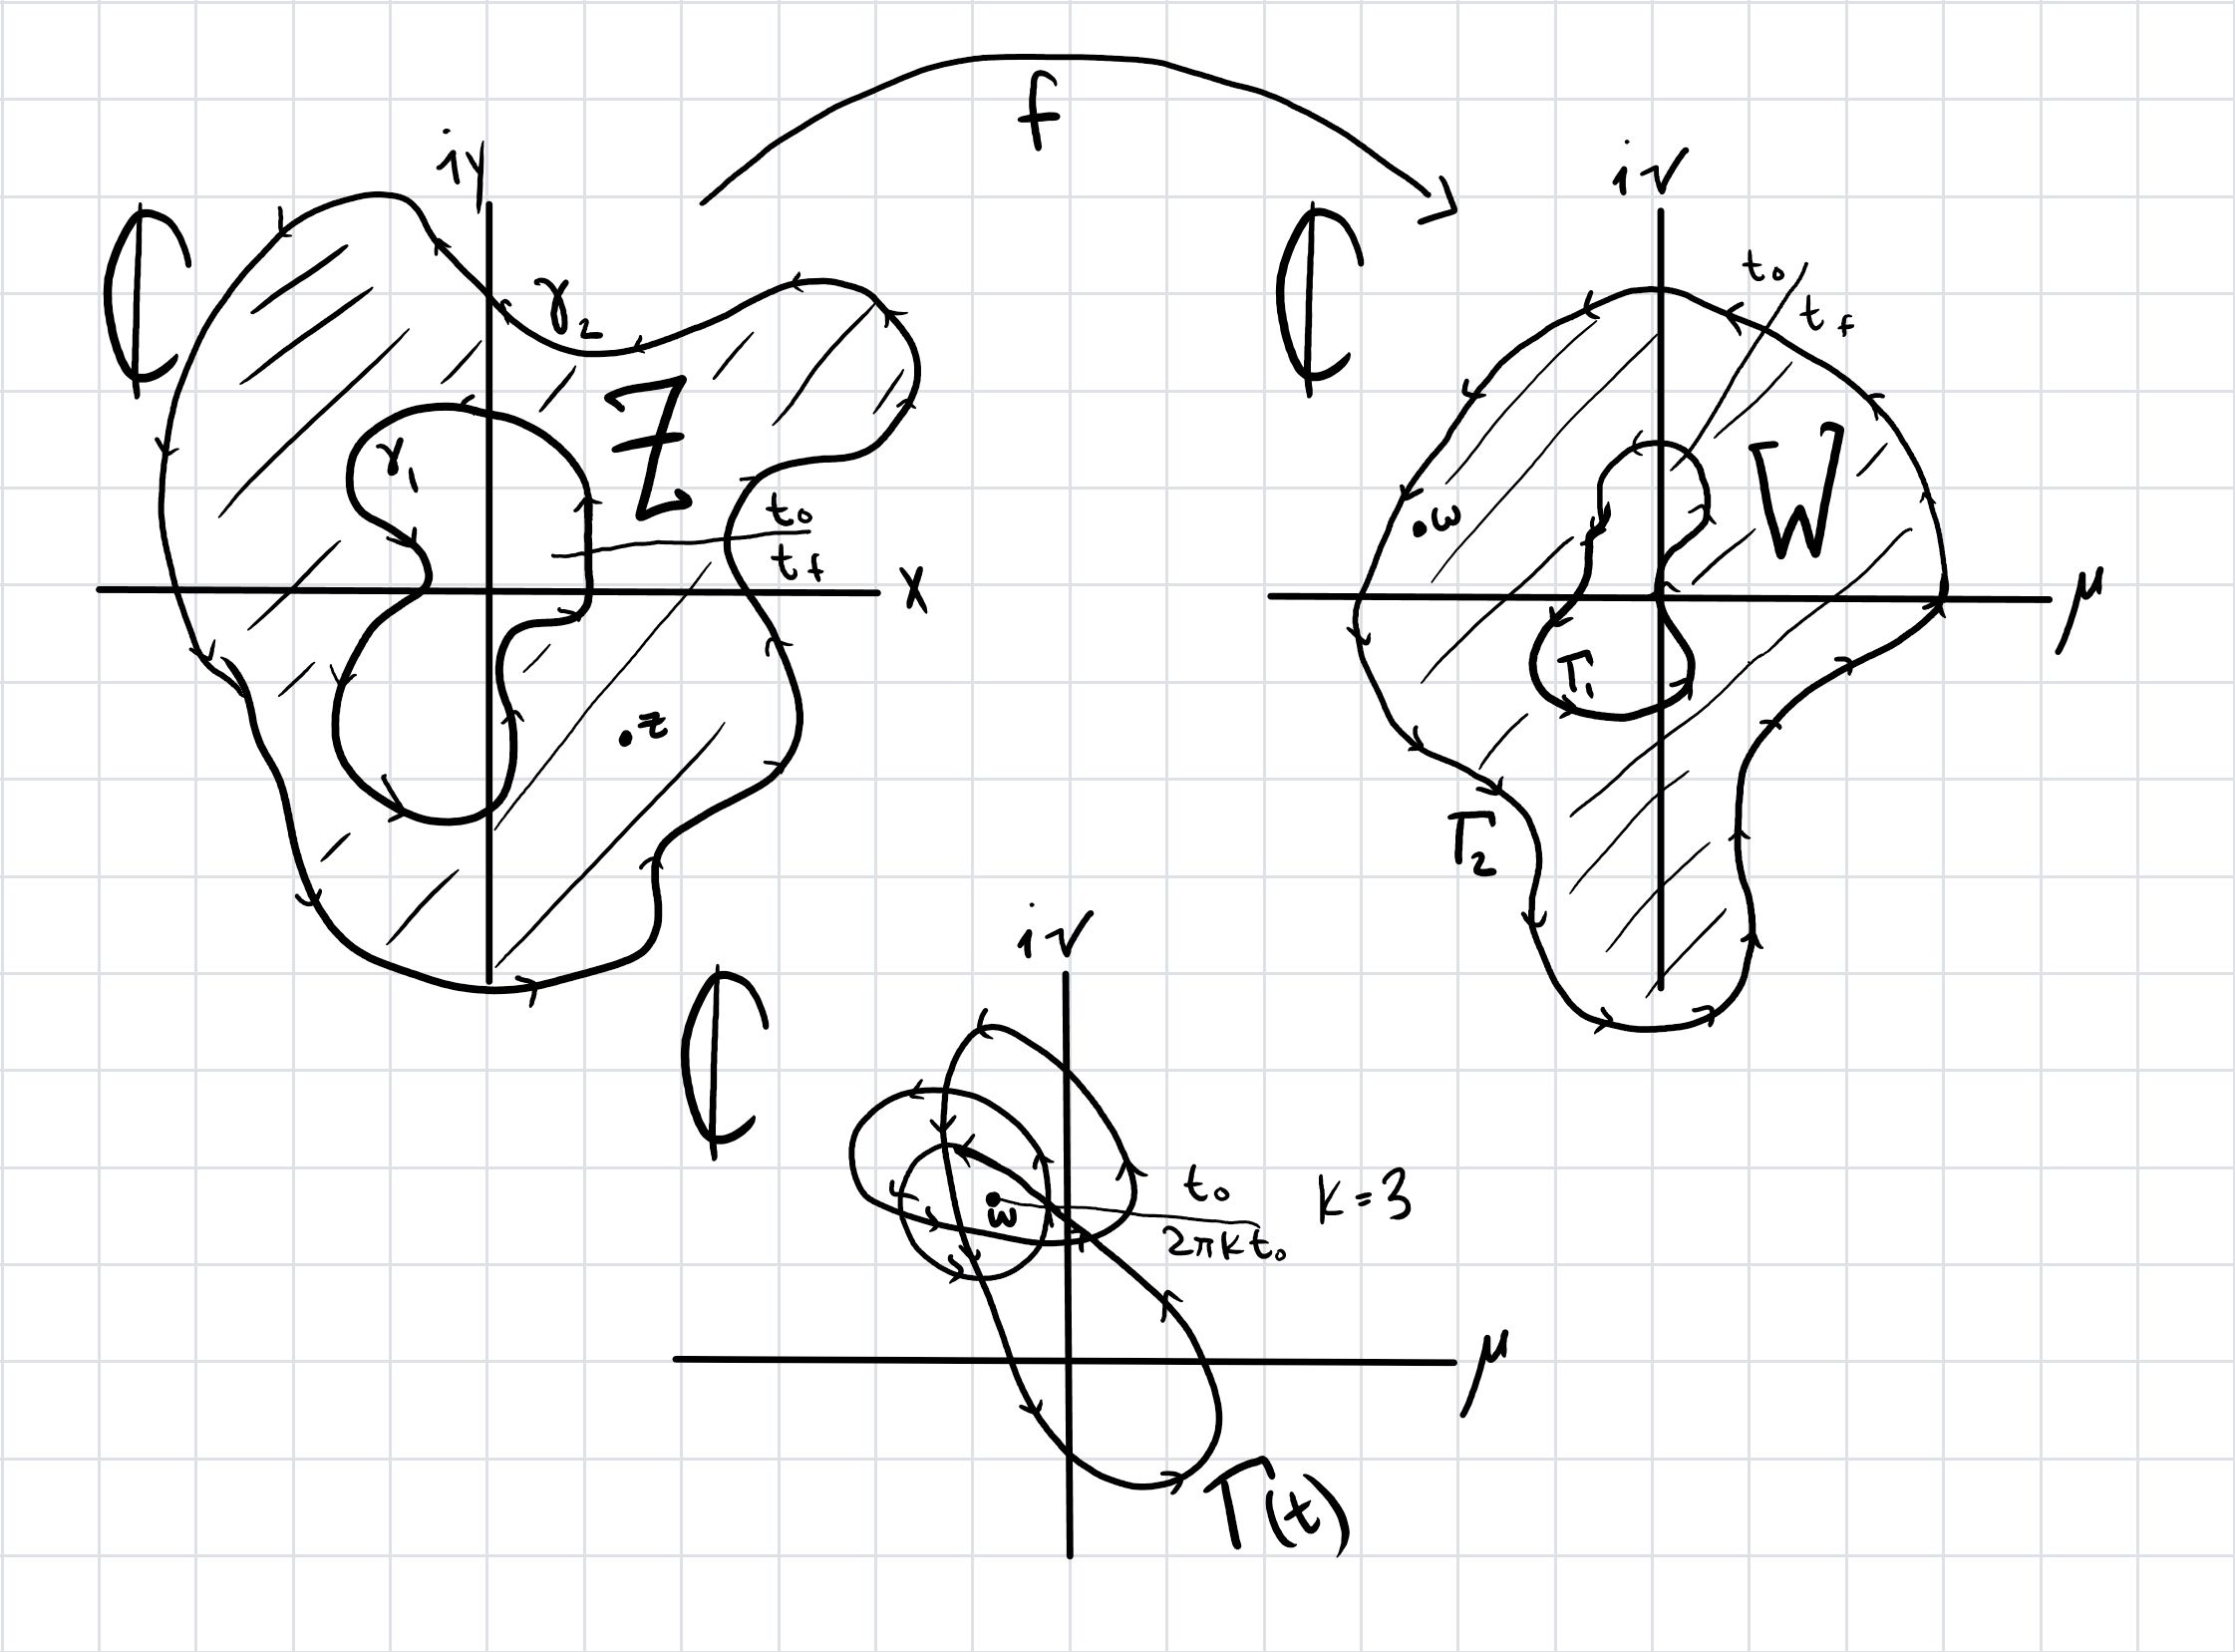
\includegraphics[width=1\textwidth]{C:/Users/cason/OneDrive - Umich/Math/CV/Project (Geometry & Mapping w C)/Parameterization.png}
      \caption{\label{C:/Users/cason/OneDrive - Umich/Math/CV/Project (Geometry & Mapping w C)/Parameterization.png}
      Illustrated here are simple loops  $ \gamma_{1}(t),\gamma_{2}(t) $ which are shown mapped by $ f $ to $ \Gamma_{1}(t),\Gamma_{2}(t) $. Below is a curve $ \Gamma(t) $, 
	looping around the point $ w $ three times, with a winding number of $ k = 3 $.}

\end{figure}

\begin{figure}

      \centering
      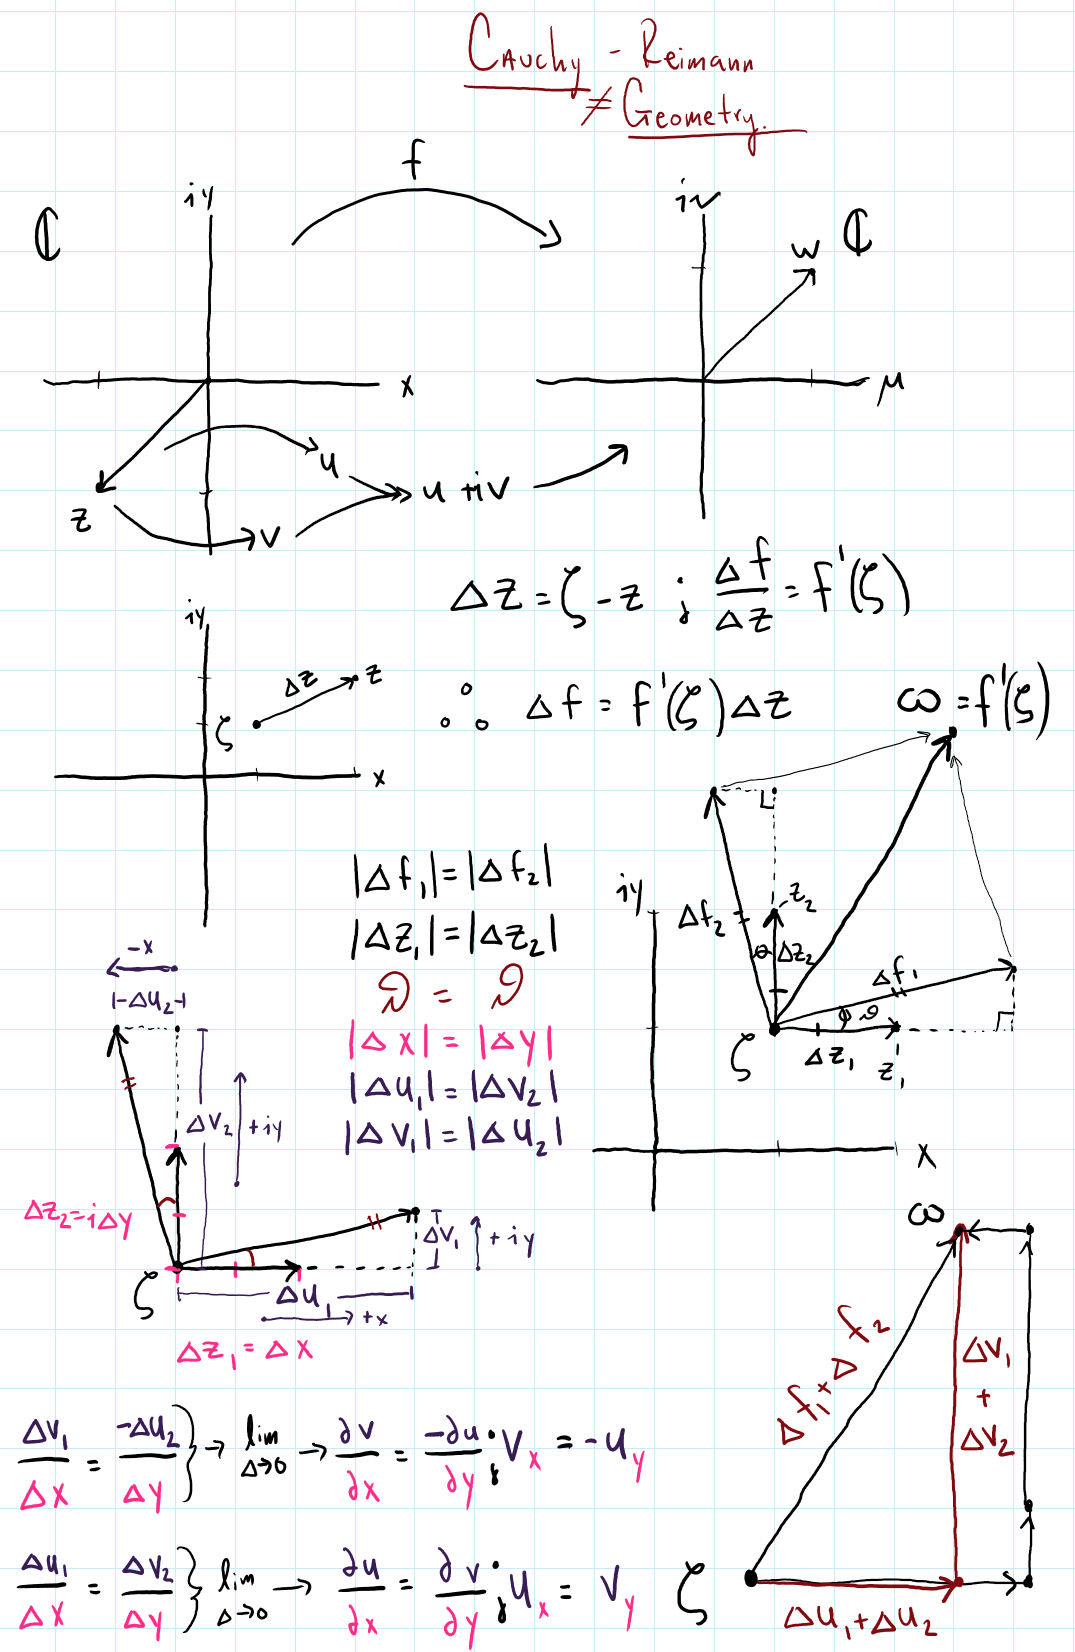
\includegraphics[width=.72\textwidth]{C:/Users/cason/OneDrive - Umich/Math/CV/Project (Geometry & Mapping w C)/CRG.png}
      \caption{\label{C:/Users/cason/OneDrive - Umich/Math/CV/Project (Geometry & Mapping w C)/CRG.png}
      Illustrated here is first a point $ z $, which when input into the $ f $ machine will output $ w $. 
      Second, a point $ \zeta $ replaces $ z $ and is input into the $ f' $ machine, with output $ \omega $. 
      At this point it is necessacray to consider $ \zeta $ in the $ u,iv $ plane. 
      $ \vartriangle z_{1} = \vartriangle x $ and $ \vartriangle z_{2} = \vartriangle y $. 
      These are the changes in the real and imaginary input respective point $ z_{1} $ and $ z_{2} $ are chosen to specifcally move along these axis. 
      Notice $ u(x,y) + iv(x,y) = \mu + \nu $, $ \vartriangle u_{1,2} $ will move along the real axis, while $ \vartriangle v_{1,2} $ will move along the imaginary axis.
      First taking ratios of $ \frac{\vartriangle u,v_{1}}{\vartriangle x} $ and $ \frac{\vartriangle u,v_{2}}{\vartriangle y} $ then taking the limit we arrive at the $ (C.R) $ equations.
      Do notice that $ \vartriangle u_{2} $ travels along the negative real axis, hence the attributed sign.} 

\end{figure}

\begin{figure}

      \centering
      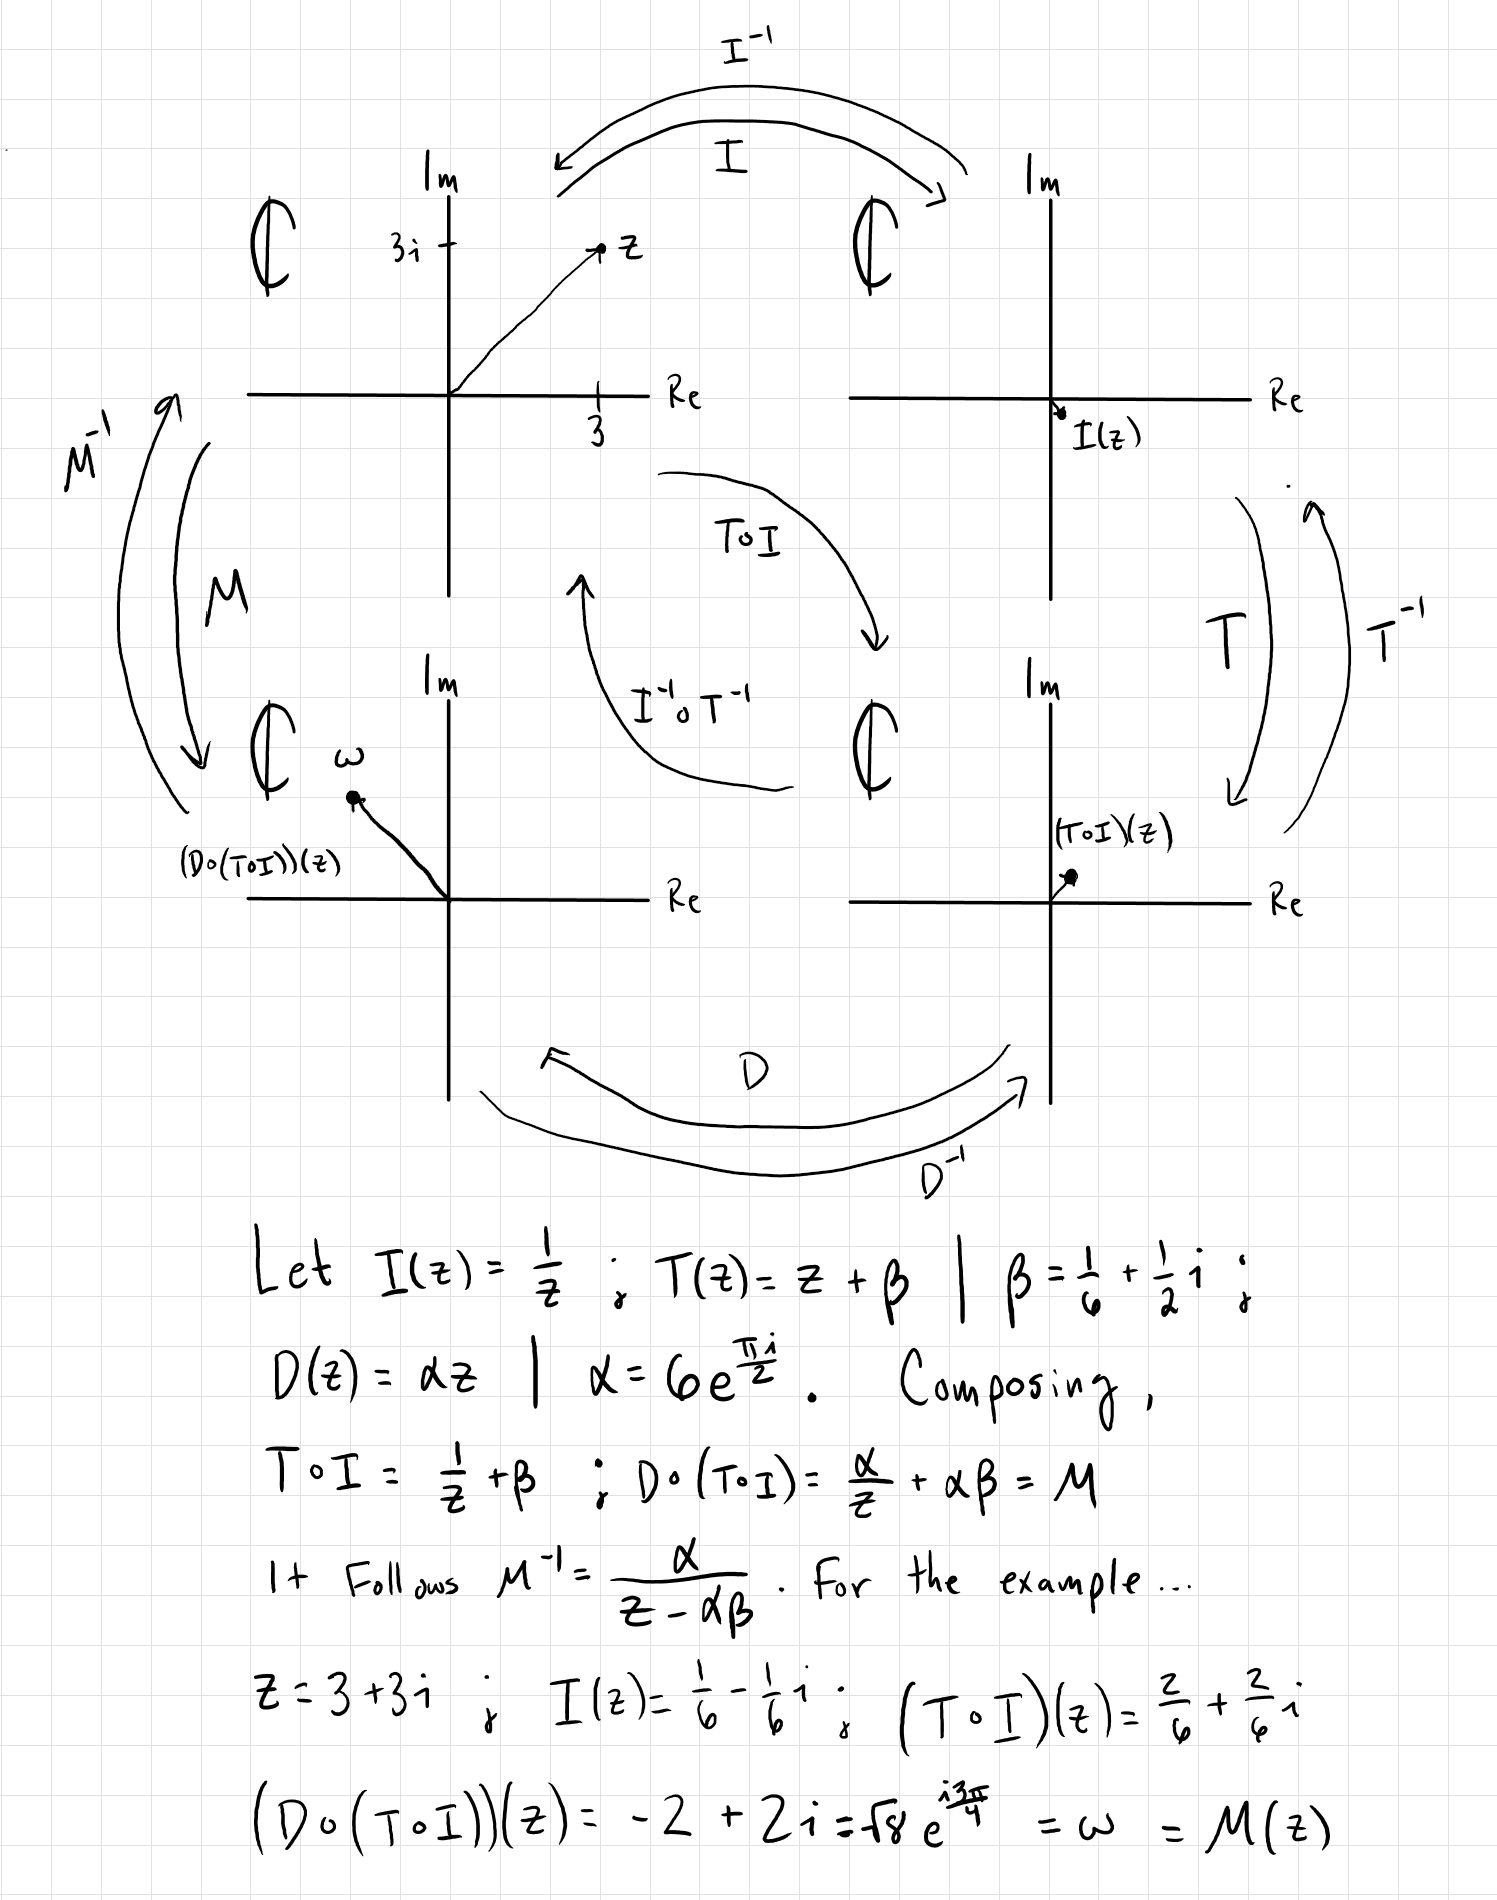
\includegraphics[width=1\textwidth]{C:/Users/cason/OneDrive - Umich/Math/CV/Project (Geometry & Mapping w C)/Mobius.png}
      \caption{\label{C:/Users/cason/OneDrive - Umich/Math/CV/Project (Geometry & Mapping w C)/Mobius.png}
      Illustrated here is the geometric movement involved in a $ m\ddot{o}bius $ transformation, 
      seen as the composition of an inversion, translation, and dialation, we visually see that there exists an inverse function. 
      While this is only for one point $ z $, we can perform the same operation on a curve $ \gamma $.}

\end{figure}

\begin{figure}

      \centering
      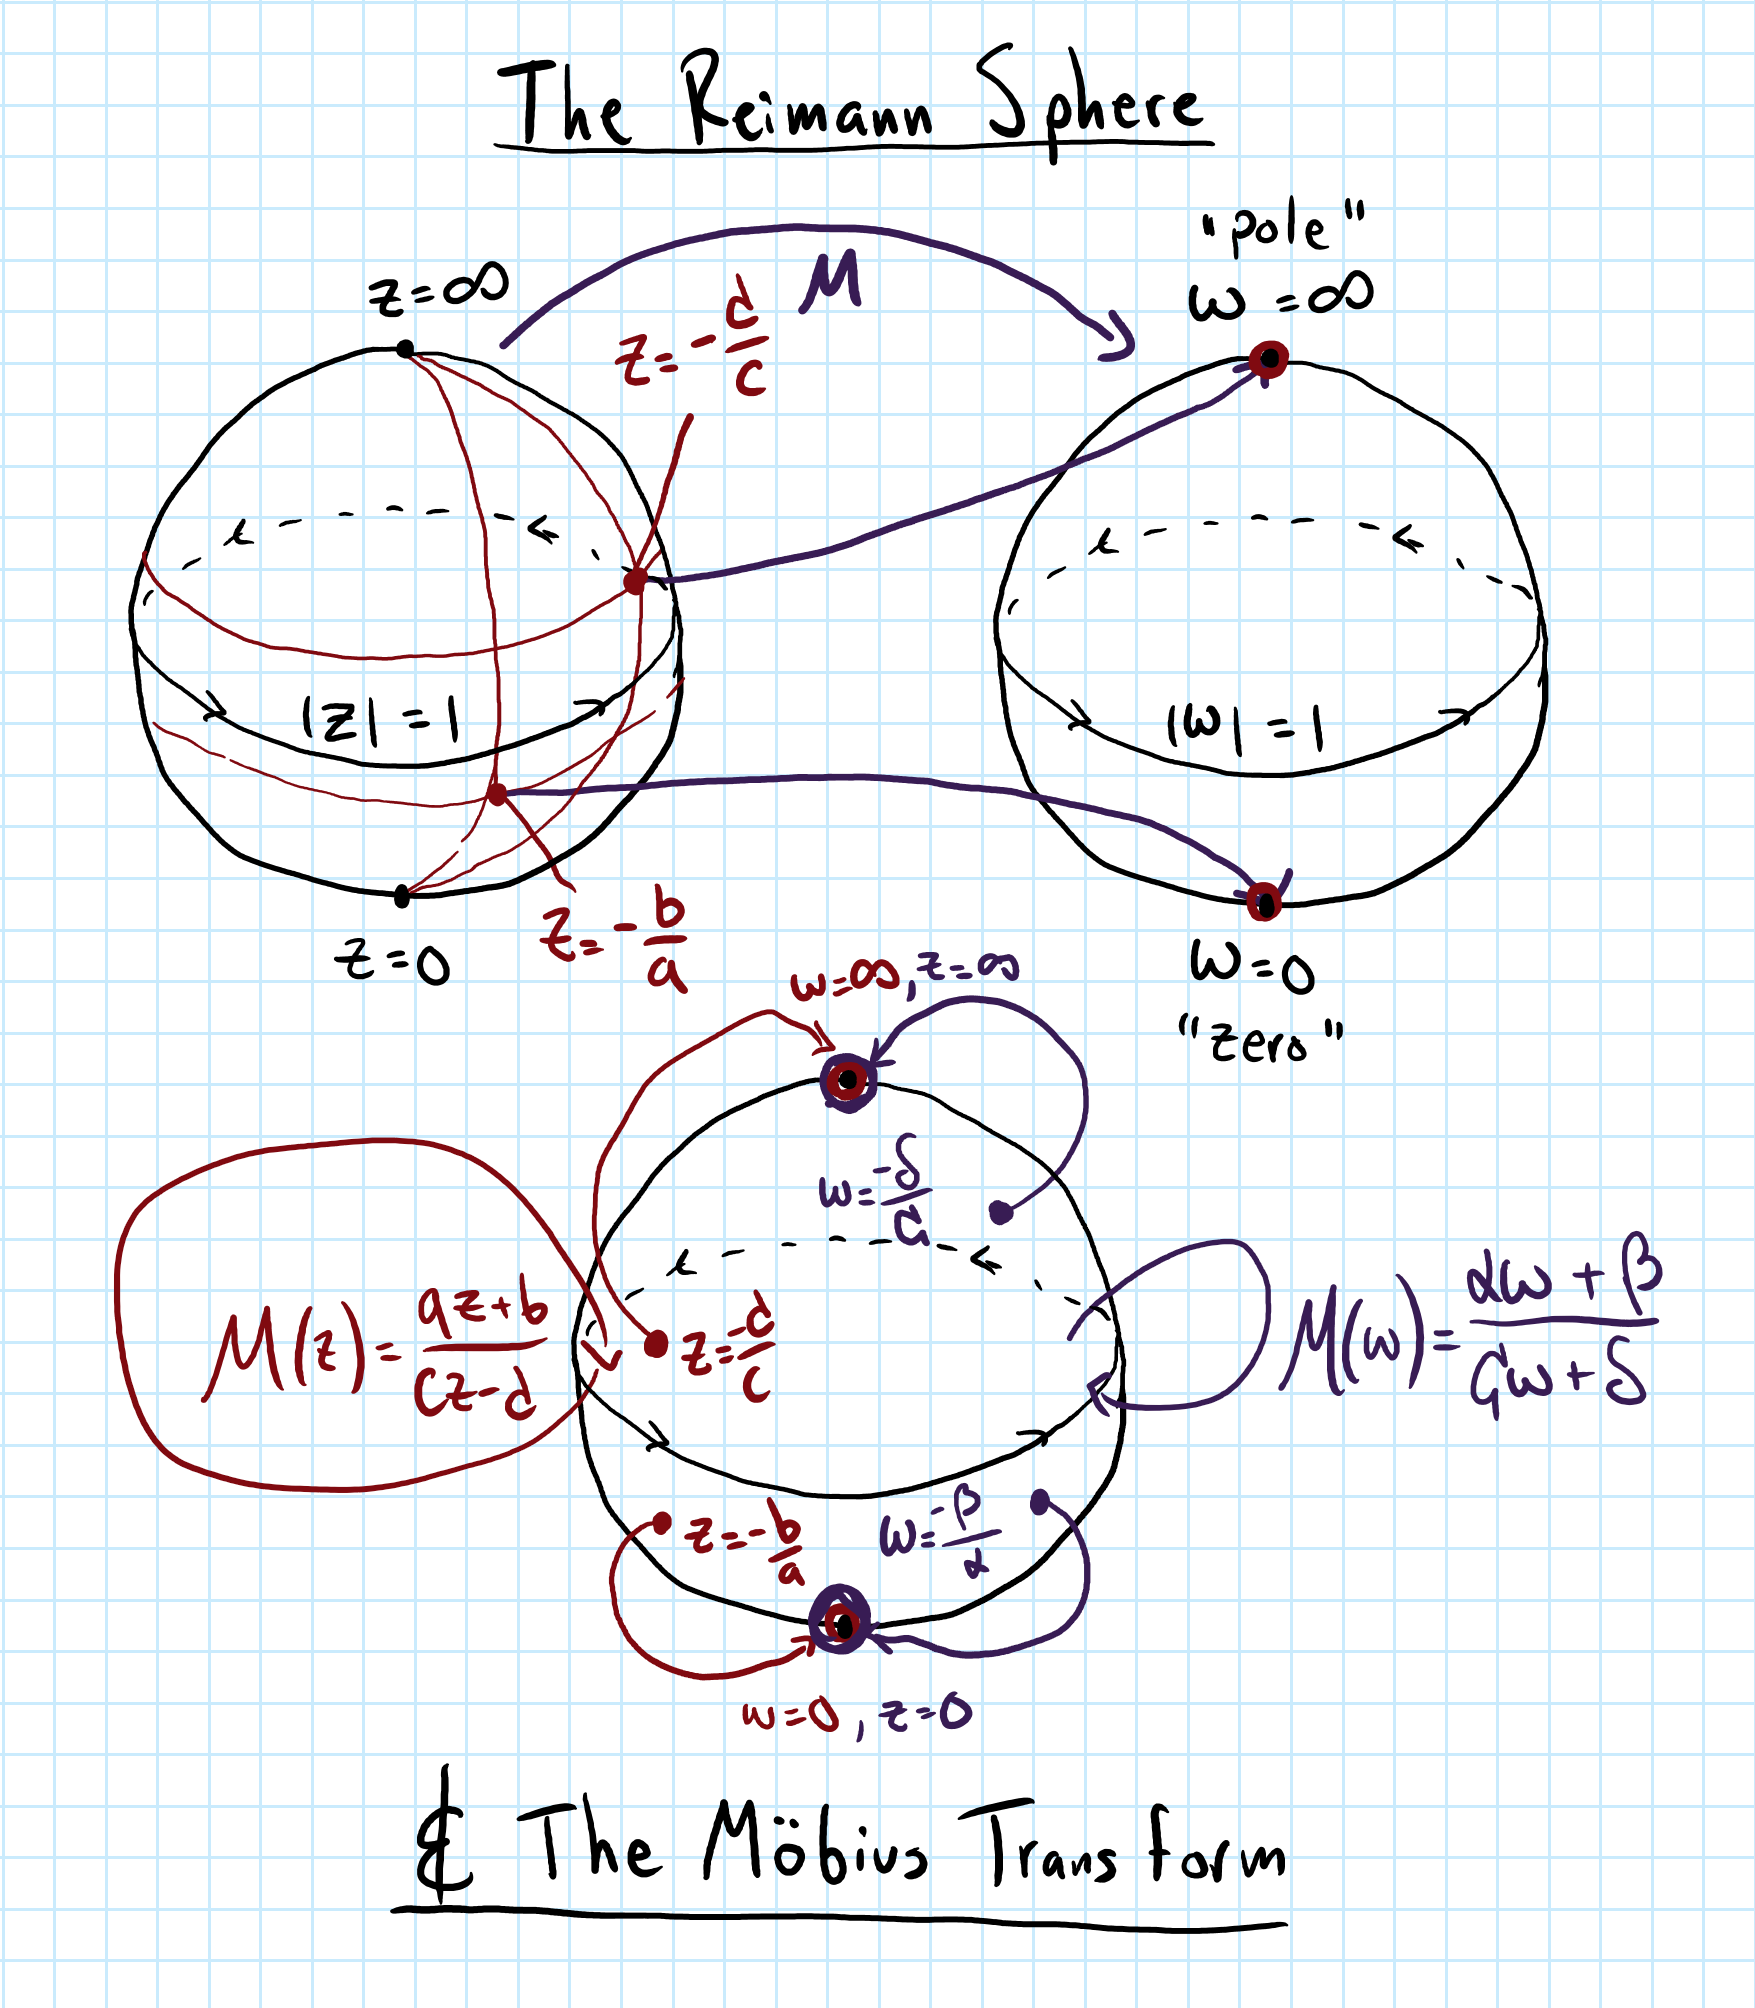
\includegraphics[width=1\textwidth]{C:/Users/cason/OneDrive - Umich/Math/CV/Project (Geometry & Mapping w C)/Reimann.png}
      \caption{\label{C:/Users/cason/OneDrive - Umich/Math/CV/Project (Geometry & Mapping w C)/Reimann.png}
      Illustrated here is a visual interpretation of the $ m\ddot{o}bius $ transformation 
      as a function that maps the surface of the Reimann spehere to the surface of the Reimann sphere.}

\end{figure}

\begin{figure}

      \centering
      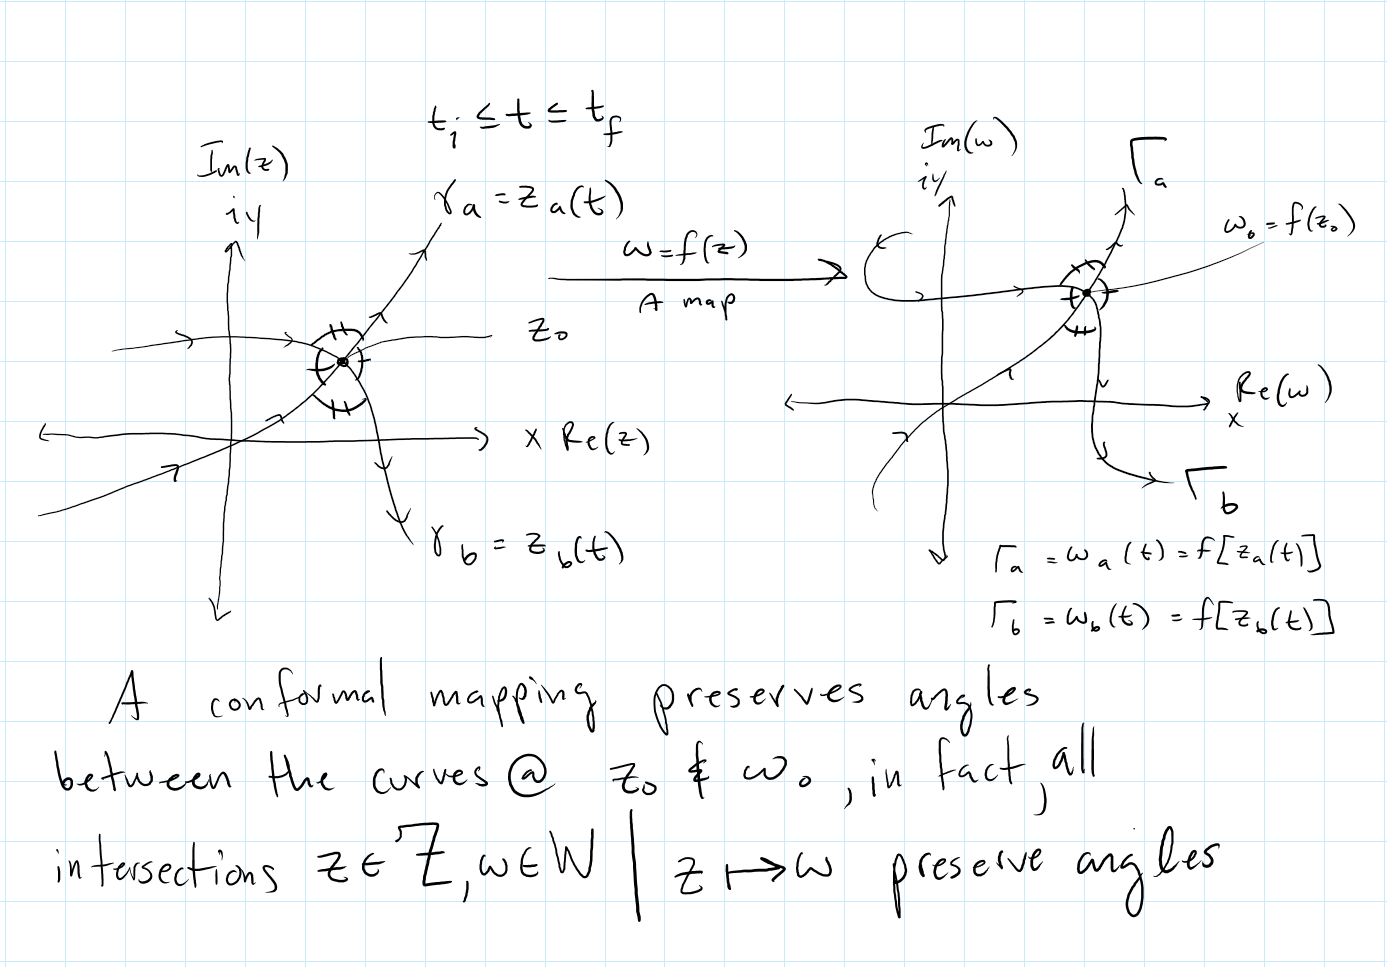
\includegraphics[width=1\textwidth]{C:/Users/cason/OneDrive - Umich/Math/CV/Project (Geometry & Mapping w C)/Angles.png}
      \caption{\label{C:/Users/cason/OneDrive - Umich/Math/CV/Project (Geometry & Mapping w C)/Angles.png}
      Illustrated here are two curves $ \gamma_{1,2} $ that map to $ \Gamma_{1,2} $ in a specific way, 
      such that the angles between the intersecting curves are preserved at the points $ z_0 $ and $ w_0 $.}

\end{figure}

\begin{figure}

      \centering
      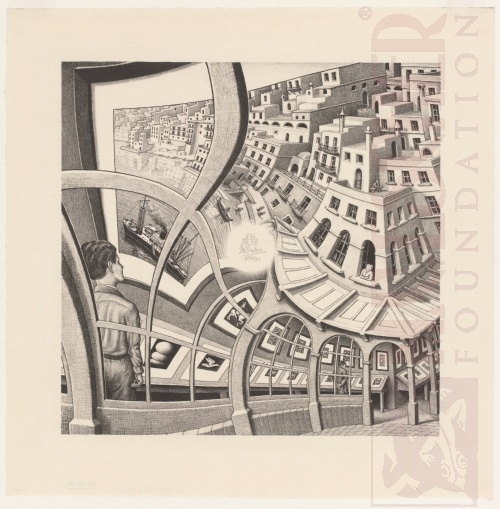
\includegraphics[width=1\textwidth]{C:/Users/cason/OneDrive - Umich/Math/CV/Project (Geometry & Mapping w C)/Escher.jpg}
      \caption{\label{C:/Users/cason/OneDrive - Umich/Math/CV/Project (Geometry & Mapping w C)/Escher.jpg}
      M. C. Escher: "Prentententoonstelling" (1956); Copyright 2003 Cordon Art B.V.-Baarn-Holland. All rights reserved}

\end{figure}

\end{document}

%Comments - April 2021 Complex Analysis Research Paper%